%%% template.tex
%%% 
%%% This LaTeX source document can be used as the basis for your technical
%%% paper or abstract. Regardless of the length of your document, the commands
%%% are all the same.
%%% 
%%% The "\documentclass" command is the first command in your file. If you want to 
%%% prepare a version of your article with line numbers - a "review" version - 
%%% include the "review" parameter:
%%% \documentclass[review]{acmsiggraph}
%%% 

\documentclass{acmsiggraph}

\usepackage{amsmath}
\usepackage{amssymb}
\usepackage{graphicx}
\usepackage{color}
\usepackage[boxed, ruled]{algorithm2e}

%%% Title of your article or abstract.

\title{Image-based Popup Craft Design via MIP Optimization}

\author{Chen Liu\thanks{chenliu@wustl.edu}}
\pdfauthor{Chen Liu}

%%% Used by the ``review'' variation; the online ID will be printed on 
%%% every page of the content.

%\TOGonlineid{45678}

% User-generated keywords.

%\keywords{radiosity, global illumination, constant time}

% With the "\setcopyright" command the appropriate rights management text will be added
% to your document.

% \setcopyright{none}
% \setcopyright{acmcopyright}
% \setcopyright{acmlicensed}
%\setcopyright{rightsretained}
% \setcopyright{usgov}
% \setcopyright{usgovmixed}
% \setcopyright{cagov}
% \setcopyright{cagovmixed}
% \setcopyright{rightsretained}

% The year of publication in the "\copyrightyear" command.

%\copyrightyear{2016}

%%% Conference information, from the completed rights management form.
%%% The "\conferenceinfo" command has two parameters: 
%%% - conference name
%%% - conference date and location
%%% The "\isbn" field includes the year and month after the article ISBN.

%\conferenceinfo{SIGGRAPH 2016 Posters}{July 24-28, 2016, Anaheim, CA} 
%\isbn{978-1-4503-ABCD-E/16/07} 
%\doi{http://doi.acm.org/10.1145/9999997.9999999}

\begin{document}

%%% This is the ``teaser'' command, which puts an figure, centered, below 
%%% the title and author information, and above the body of the content.

\teaser{
  
\includegraphics[height=1.5in]{Figures/teaser}
  \caption{(a) Input 2D shape and its segmentation. (b) Generated cuts and folds. (c) 3D pop-up rendering.}
}

\maketitle

\begin{abstract}

  In this project, we focus on automatic popup craft design with the problem setting from \cite{liu2014image}. But instead of using the greedy method used in \cite{liu2014image}, we use non-linear optimization to optimize the design globally. The optimization formulation is designed such that an optimal solution is a popup design which 1) follows the input shape, 2) is foldable, and 3) is connected, and 4) is stable (See Section \ref{introduction}).
\end{abstract}

% 
% The code below should be generated by the tool at
% http://dl.acm.org/ccs.cfm
% Please copy and paste the code instead of the example below. 
% 
% \begin{CCSXML}
%   <ccs2012>
%   <concept>
%   <concept_id>10010147.10010371.10010382</concept_id>
%   <concept_desc>Computing methodologies~Image manipulation</concept_desc>
%   <concept_significance>500</concept_significance>
%   </concept>
%   <concept>
%   <concept_id>10010147.10010371.10010382.10010236</concept_id>
%   <concept_desc>Computing methodologies~Computational photography</concept_desc>
%   <concept_significance>300</concept_significance>
%   </concept>
%   </ccs2012>
% \end{CCSXML}

% \ccsdesc[500]{Computing methodologies~Image manipulation}
% \ccsdesc[300]{Computing methodologies~Computational photography}

% % 
% % End generated code
% % 

% % The next three commands are required, and insert the user-generated keywords, 
% % The CCS concepts list, and the rights management text.
% % Please make sure there is a blank line between each of these three commands.

% \keywordlist

% \conceptlist

% \printcopyright

\section{Introduction} \label{introduction}
Popup craft, introduced by Masahiro Chatani in 1980, is a design of cuts and folds on a single piece of paper. Complex and interesting structure pops up when the paper is opened. The special structure of a popup craft makes it appealing but hard to design. In this work, we seek an automatic design method via an optimization process. 

Given either a Vector image or a scalar image, we first segment it to get a segmentation image $\mathcal{S}$ which stores a segment index for each pixel. Based on $\mathcal{S}$, we find initial fold lines between pair of different segments. Given these initial fold lines, we find other fold line candidates in a sense that a new fold line candidate affects the topology of initial fold lines. With all the fold lines as candidates, we determine their activeness, convexity, and positions in an optimization framework. By adding auxiliary variables and constraints, we enforce an optimal solution to be a popup craft design with satisfactory properties. First, a popup craft must be foldable, which means it can be opened and folded without breaking its geometry (see \cite{li2010popup} for more details). Second, a popup craft is more appealing when it is stable, which means the structure is stable when two border of the paper is holded (see \cite{li2010popup} for more details). Third, because the number of segments of the popup craft is limited in our image-based problem setting, the connectivity, which enforces there is only one connected structure in the popup craft, becomes important. Fourth, the popup craft should follow the input shape.
\section{Related Work}

Due to rigid paper crafting constraints, the OA design process is often time consum- ing and requires considerable skills. Several computer-aided design tools have been developed to provide a virtual design environment and assist the design process (see \cite{mitani2004computer} and the references therein). However, the ultimate placement of cuts and folds still depends on the user, posing the design process trouble- some and highly skill-demanding. To further simplify OA design, Li et al.~\cite{li2010popup} proposed a fully automatic algorithm to convert building models to paper architectures. Le et al.\cite{le2014surface} presented a surface-and-contour-preserving method to pop up 3D models with more freeform shapes. Liu et al.\cite{liu2014image} proposes an image-based approach but the greedy approach fails in many cases.
\section{Popup Graph}
We define two types of popup graphs based on three types of units: \textit{segments}, \textit{regions}, and \textit{fold line candidates}. \textit{Segments} come directly from input image segmentation. Inside each segment, there are usually multiple \textit{regions}, each of which contains one fold line candidate. A fold line candidate is potentially effective fold line in the final design. There are two types of \textit{fold line candidates}. \textit{Intersection fold line candidates} come the intersection between two neighboring \textit{segment}. And \textit{region fold line candidates} come from each region. We first segment the input image (see section \ref{image_segmentation}), then find \textit{intersection fold line candidates} (see section \ref{intersection_fold_line_candidates}), and then find \textit{regions} and corresponding \textit{region fold line candidates} (see section \ref{region_fold_line_candidates}. We incorporate all information to build two types of graphs as explained in \ref{popup_graph_structure}.  Three units and two popup graphs are illustrated in Figure \ref{fig:graph}.

\subsection{Image Segmentation} \label{image_segmentation}
We take either a vector image or a scalar image as input. For a vector image, we read the segment information from the image directly. For a scalar image, we segment the image using Watershed algorithm.

\subsection{Find Intersection Fold Lines Candidates} \label{intersection_fold_line_candidates}
For a popup craft, fold lines serve as joints connecting two patches. Most fold lines lie between two neighboring segments and connect them. For any given pair of neighboring fold lines, there could be arbitrary number of fold lines with arbitrary position along the intersection. Ideally, we want one fold line candidate for each possible position, but then the optimization becomes intractable. The opposite extreme is to have only one fold line candidate but allows it to appear anywhere along the intersection. In practice, we first divide the intersection into multiple parts such that it is unlikely for each part to contain more than one fold lines. Then we assign one fold line candidate for each part. We define a \textit{slope} as a part of the intersection where $x$ is monotonically increasing or decreasing over $y$ as shown in Figure \ref{fig:valley}. We find that there is usually at most one fold line in each \textit{slope}. But dividing directly by \textit{slopes}, we borrow the idea of max-suppression. We first pick the position with the best score (defined below) and then suppress positions in the same slope (in cases where the picked position is at the intersection point of two slopes, positions in both slopes will be suppressed). We repeat the process for the remaining positions until are positions are considered. Each picked position will be the desirable position for one fold line candidate and corresponding suppressed positions will be the possible positions for this candidate.

To define the score for a fold line candidate at given position, we look at a local window around that position. The size of the window has clear physical meanings. When we make actual popup crafts out of a hard paper, a fold line has to be long enough so that it connects two patch stably. Also, we want patches beside it to be wide enough so that the fold line is easy to fold by hand. The height of the local window is chosen to be the minimal fold line length and the width of the local window is chosen to be twice of the minimal patch width beside a fold line. For a fold line $f$ to appear at pixel $p$, denote its left segment as $s_l$ and its right segment as $s_r$, the score of the fold line $f$, is determined as \ref{equ:goodness}.
\begin{equation}
  S(f, p, s_l, s_r) = \frac{|W_l(p) \cap R(s_l)| * |W_r(p) \cap R(s_r)|}{(0.5 H^f W^f)^2}
  \label{equ:goodness}
\end{equation}

% There are two key parameters in this task. $H^f$ is the desirable height of the local window of a fold line and $W^f$ is the desirable width of the local window. Here, the local window is simply a rectangle region on the image. For a pixel $p$ in $\mathcal{S}$, we look at its local window $W(p)$ with height $H^f$ and width $W^f$. There could be more than one segments $W(p)$ and for each pair of them which are adjacent, we can put a fold line between them at $p$. For any such pair, there are two options in terms of which one is left (right). For each option, denote the left segment as $s_l$ and the right segment as $s_r$, the score of the fold line $f$ between them at $p$ is determined as \ref{equ:goodness}.
% \begin{equation}
%   S(f, p, s_l, s_r) = \frac{|W_l(p) \cap R(s_l)| * |W_r(p) \cap R(s_r)|}{(0.5 H^f W^f)^2}
%   \label{equ:goodness}
% \end{equation}
% Here $W_l(p)$ and $W_(p)$ are the left half and right half of $W(p)$ respectively, and $R(s)$ is the region of $s$ on the image domain. The intuition for this equation is for a fold line to be more reliable, it should have more left segment pixels on its left and more right segment pixels on its right. The score is in $[0, 1]$ by its definition.

% After we iterated over all pixels and found all such fold line candidates, we use a greedy strategy to filter out the ones with lower score. In filtering process has two stages. In the first stage, the competition is among fold lines between same pair of segments with same direction. For each pair of segments with same direction, we first collect all the fold lines between them and corresponding pixels. We first choose to keep the one with the highest score, and then filter our all the fold lines which can be reached by going either to left or right along the segment boundary starting from the center point of this fold line. We repeat this process for remaining fold lines until all fold lines are considered. The intuition is to choose one fold line with the highest score in each ``valley'' (a ``valley'' is defined vertically on the boundary between this two segments). (See figure \ref{fig:valley}.)

% \begin{figure}[h]
%   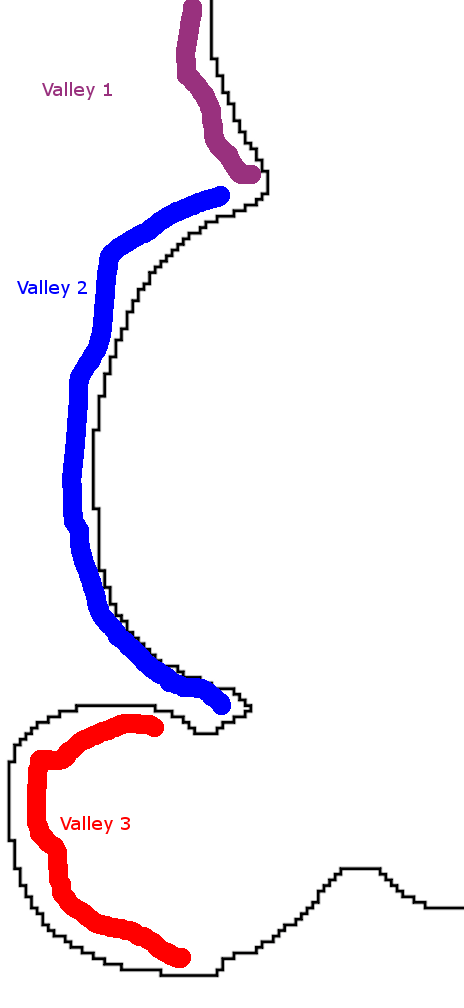
\includegraphics[width = 0.2\textwidth]{Figures/valleys}
%   \caption{Illustration of valleys. Valleys are defined for same pair of patches and each valley could contain at most one fold line.}
%   \label{fig:valley}
% \end{figure}


% In the next stage, the competition is among fold lines between same pair of segments with different direction. The intuition here is for some segment pairs, we are certain that which one should appear left (right), and we want to remove the fold line which indicates opposite direction. The process is conducted by checking two fold line between same segment pair but with different direction. If they can reach each other by going up or down along the segment boundary, we remove the one with lower score.

% After the filtering process, initial fold lines are already pretty nice. We further remove some fold lines if they are too close to some other fold lines with higher score. And for background segment, we only use one fold line candidate.

\subsection{Find Region Fold Line Candidates} \label{region_fold_line_candidates}
Although most fold lines lie on the intersection betweeo segment pairs, some segments themselves have to be folded to make the popup craft foldable (e.g. the fold lines on the arm of the bear example). A segment can be folded for arbitrary number of times at arbitrary position inside the segment. Similar with finding intersection fold line candidates, we divided the segment into multiple regions and associate one fold line candidate with each region. A fold line folds a segment into two halves, and at the same time, divides intersection fold line candidates into two groups. A region is defined such that whereever a fold line is put in the region, the division of intersection fold line candidates does not change. Then it is reasonable to add only one fold line candidate in each region and allows it to appear at any position in the region.

% After finding all initial fold lines, we can define the topology of initial fold lines on each segment. Here we look at the topology for each segment independently because a new fold line candidate only affect one segment. For segment $s$, we define the topology simply based on the connectivity of its initial fold lines on $R(s)$. We separate $R(s)$ into sub-regions in a sense that the topology is the same whereever a new fold line is put in the sub-region. We put a new fold line candidate in each sub-region (not for the ones which has no initial fold lines on its left or right).

\subsection{Structure and Properties} \label{popup_graph_structure}
A segment-based popup graph has \textit{segments} as nodes and \textit{intersection fold line candidates} as edges connecting two segments. A segment-based popup graph has the following properties:

\textbf{Background Enclosing: } A popup graph has a background segment enclosing all other segments.

\textbf{Directed Acyclic Graph (DAG): } We denote the direction of an edge (fold line candidate) as from its left segment to its right segment. Then the graph excluding the background segment is a DAG.

\textbf{Source and Sink: } The background segment serves as both the source and the sink for all paths.

A candidate-based popup graph has both types of \textit{fold line candidates} as nodes, and their neighboring relations as edges. Two fold lines are regarded as neighbors only when they belong to the same segment and there is no fold line between them. A candidate-based popup graph has the same set of properties:

\textbf{Background Enclosing: } The background segment has one region fold line candidate called \textit{background fold line} which is always active. The \textit{background fold line} divides the background segment into two halves. We call these two halves \textit{left background patch} and \textit{right background patch}. This corresponds to the two halves of most blessing cards.

\textbf{Directed Acyclic Graph (DAG): } The left-right orientation between fold line candidate pairs is well-defined and the the graph excluding the background fold line is also a DAG.

\textbf{Source and Sink: } The background fold line serves as both the source and the sink for all paths.


% \subsection{Retrieve Popup Graph Information} \label{popup_graph_information}
% We can define the graph based on all fold line candidates. A fold line neighbor pair $(f_l, f_r)$ is found by looking at neighbor pixels. (Note that each fold line candidate occupies a region $R(f)$ on the image domain.) For $f_s$ and $f_t$ belonging to the same segment $s$, a fold line path $P(f_s, f_t)$ is defined as the sequence of fold lines of $s$ through which might affect the connectivity of $f_s$ and $f_t$. (See figure \ref{fig:path}.)

% \begin{figure}[h]
%   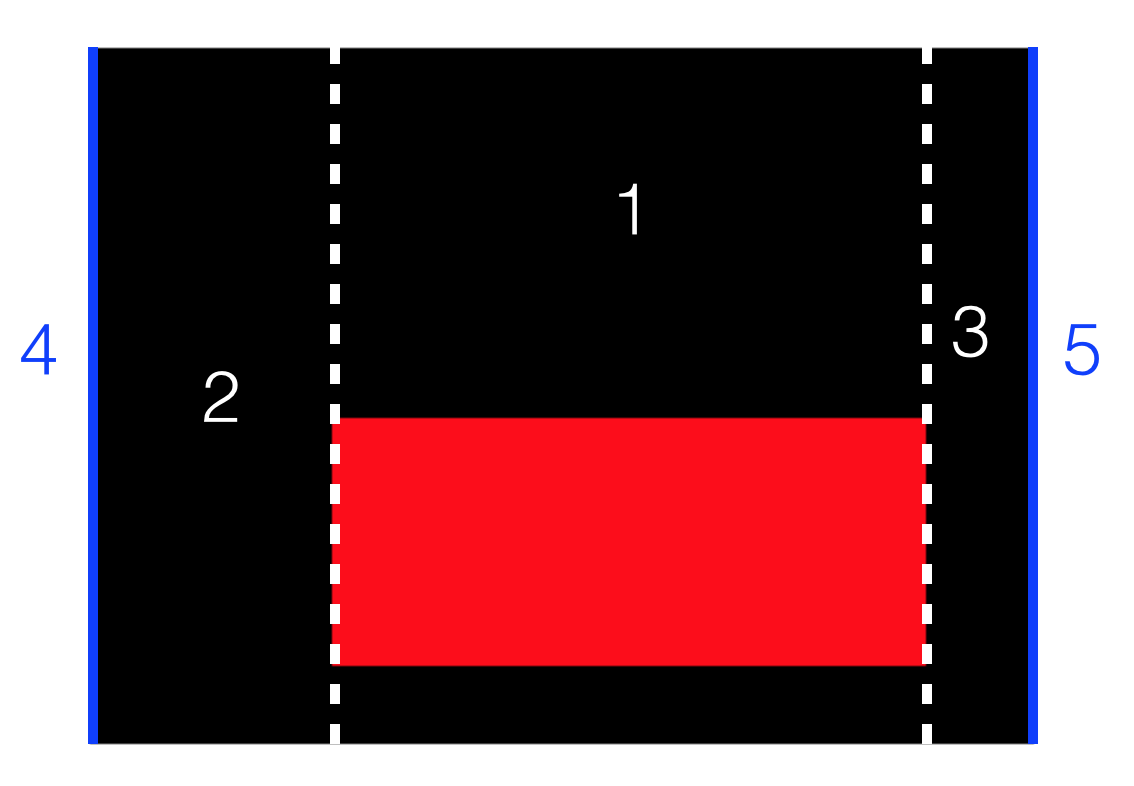
\includegraphics[width = 0.3\textwidth]{Figures/path}
%   \caption{We say fold line sequence \{2, 1, 3\} is a path between fold line 4 and fold line 5. Fold line 4 and fold line 5 will appear on the same final patch if fold line \{2, 1, 3\} are all inactive.}
%   \label{fig:path}
% \end{figure}


% We add two special fold lines, one for left image border $Lf$ and one for right image border $Rf$, to ease formulation.


\section{Optimization}
Given a popup graph family, we need to determine the following three sets of variables in order to choose the optimal popup graph.
\begin{enumerate}
\item $a(f)$: A binary variable indicating the activeness of fold line $f$.
\item $c(f)$: A binary variable indicating the convexity of fold line $f$ (whether the fold line points outwards ($c(f) = 1$) or inwards ($c(f) = 0$).
\item $p(f)$: A integer variable indicating the position of fold line $f$.
\end{enumerate}

The goal is to determine these variables so that the popup graph satisfies four key properties: foldability, connectivity, stability and consistency. Additional properties can be enforced according to user input. We can view our task as an optimization problem $G^{OPT} = optimize(\mathcal{G})$ which takes a popup graph set $\mathcal{G}$ as input and outputs the optimal popup graph:

\begin{equation}
\begin{aligned}
  G^{OPT} = & argmax_G \quad Consistency(G) \\
            & s.t. G \in \mathcal{G} \quad and \quad Foldability(G) = TRUE \quad and \quad Connectivity(G) = TRUE \quad and \quad Stability(G) = TRUE \quad and \quad User(G) = TRUE
\end{aligned}
\end{equation}
  

We formulate the optimization problem as a mxied integer programming problme. We will explain how to formulate each property as either quadratic objective terms or quadratic constraint terms and provide heuristics for making the optimization problem tractable.

\subsection{Foldability}
\textbf{Foldability Definition: }

\textbf{Variable Definition: }
We associate a set of variables $c(f)$ determining the convexity of $f$, that is . A set of variables $X(f)$ determining the X coordinate of $f$, and $Y(f)$ determining the Y coordinate of $f$.

There is $x(f) + y(f) = p_u(f)$ ($p(f) = (p_u(f), p_v(f))$).

The orientation constraints involve $c(f)$. For fold line neighbor pair $(f_l, f_r)$, there is:
\begin{equation}
  \begin{aligned}
    & c(f_l) = 1 - c(f_r) & \text{ if } a(f_r) = 1 \\
    & c(f_l) = c(f_r) & \text{ otherwise } \\
  \end{aligned}
\end{equation}

The position constraints is formed as:
\begin{equation}
  \begin{aligned}
    & x(f_l) < x(f_r) \quad & y(f_l) = y(f_r) & \text{ if } c(f_r) = 1 \\
    & x(f_l) = x(f_r) \quad & y(f_l) < y(f_r) & \text{ otherwise } \\
  \end{aligned}
\end{equation}

\subsection{connectivity}
Due to the fact that the number of segments is small in our image-based design process, we prefer one intriguing structure containing all segments instead of multiple separated simple structures.. For this reason, we enforce two type connectivity here. First, each patch should have at least one path from both left background patch and right background patch. Second, after taking background patches away, the rest graph should have only one connected component. The connectivity property is incorporated into the optimization formulation as follows.

As new fold lines will never be cut, the connectivity property is considered based on initial patches. The first type of connectivity is enforced by simply adding a constraint that each initial patch (except the background patch) has at least one active left initial fold line and one active right initial fold line. The proof is trivial as the graph has non-loop property. We re-phrase the second connectivity constraint as there exists at least one connection between any pair of patches (background patches are excluded). Here the connection exists when:

\begin{enumerate}
\item For a pair of neighboring patches, at least one fold line between them is active.
\item For a pair of non-neighboring patches, they both have connection with at least one other patch.
\end{enumerate}

Due to the symmetric definition of connection, we can simplify the constraint as there exists at least one connection between each patch and one denoted patch $s$. The denoted patch is a randomly picked non-background patch. Then we define the connection depth for each patch as the length of the shortest path to patch $s$. We use binary variable $c_{pd}$ to indicate whether patch $p$ has connection depth $d$ ($d \in [1, MAX\_DEPTH]$). Based on $c_{pd}$, the connectivity constraint is formulated as $\sum_d{c_{pd}} = 1$. According to the definition of connection, $c_{pd}$ subjects to:

\begin{equation*}
  \begin{cases}
    c_{p1} \leq \sum_{f \in F(p, s)}a(f) & \text{ If patch $p$ is a neighbor of $s$} \\
    c_{p1} = 0 & \text{ If patch $p$ is not a neighbor of $s$} \\
    c_{pd} <= \sum_{q \in N(p)}(c_{q(d-1)}\sum_{f \in F(p, q)}a(f))
  \end{cases}
\end{equation*}

Note that some patches do not have active fold lines because they lie inside another patch (see the eyes in the bear example). We call them ``island patches''. For island patches, connectivity no longer holds. For this reason, we add another set of binary variables $i(p)$ to indicate whether a patch is an island patch or not. We modify the above connectivity constraints so that they are disabled for island patches. And an island patch has no fold line, so there should be $a(f) <= 1 - i(p) \quad \forall f \in F(p)$.

\subsection{Stability}
We associate a set of binary variables $s(f)(d)$ indicating the stability of $f$ at depth $d$. Here the depth can be interpolated as the following procedure. $Lf$, $Rf$, and all fold lines on the background patches are stable at depth 0. Now if we add two patches between background patches forming a stable structure, the corresponding fold line will be stable at depth 1. We can continue to add stable structure based on current structure and the depth increases as the procedure goes on.

We use the idea of forming the popup by iteratively adding stable structure to formulate the stability constraint. That is, we check a building block at depth $d$ to see whether it is stable or not based on previous building blocks (with stability depth less than $d$).


% Note that we only consider stability for active fold lines. A key additional variable $same\_patch(f_s, f_t)$ indicates whether $f_s$ and $f_t$ are on the same final patch. $same\_patch(f_s, f_t) = 1$ when $P(f_s, f_t)$ exists and its fold lines are all inactive (meaning the patch is not folded). (See figure \ref{fig:path}.) With $same\_patch(f_s, f_t)$, we can sum up with support from all fold lines on the same patch to form constraints as $\#(f_t) <= \sum_s{*(f_s)c(f_s, f_t)}$ (see figure \ref{fig:support} for details).

% \begin{figure}[h]
%   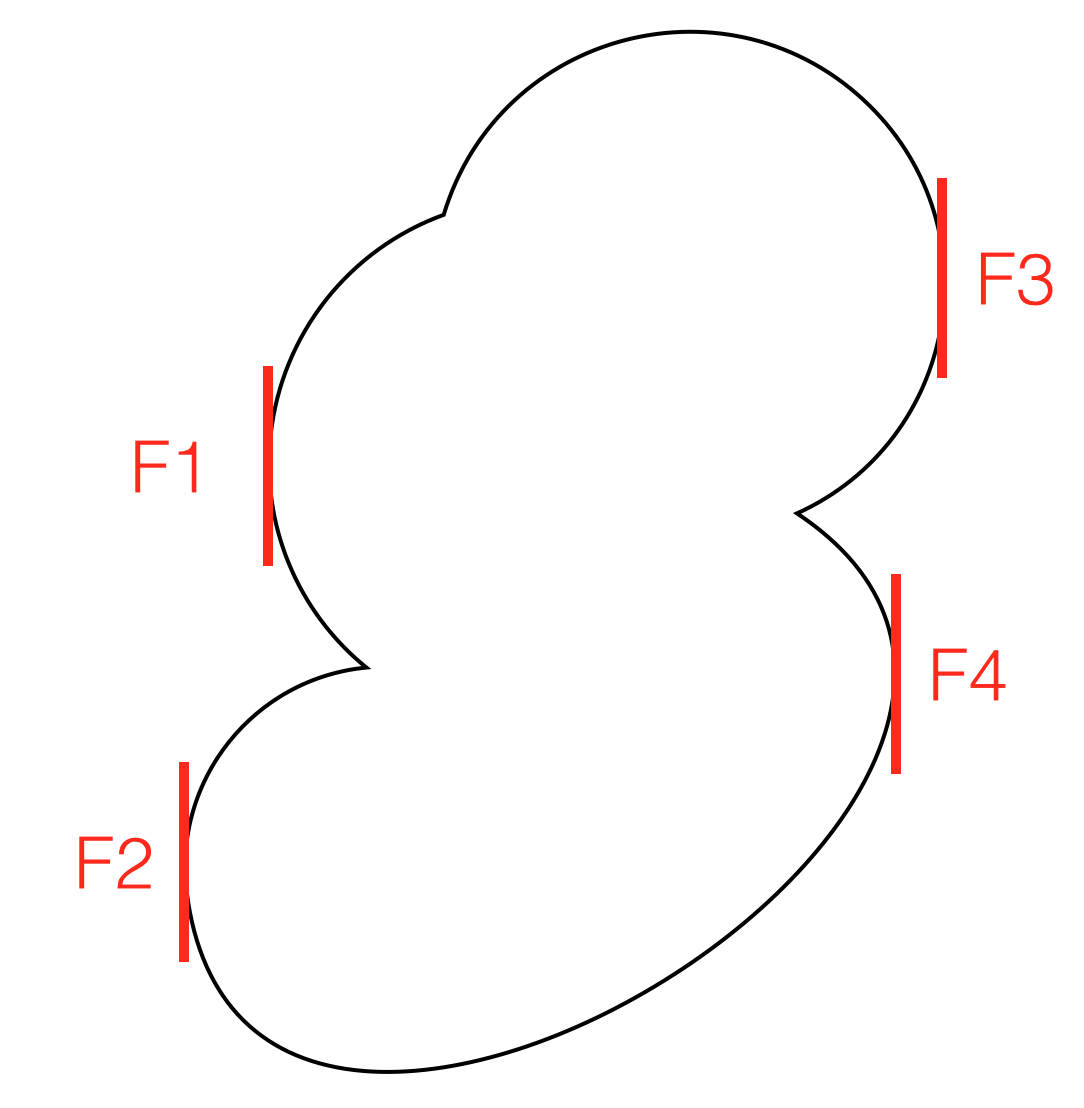
\includegraphics[width = 0.3\textwidth]{Figures/support}
%   \caption{Suppose these four fold lines are on the same final patch (determined by same\_patch($f_i$, $f_j$) = 1). Then the attribute for each fold line results from the support from all these four fold lines. To be more specific, for these four fold lines, we have the following. 1) If two or more fold lines are stable, then other fold lines are also stable. 2) If one fold line is stable, then other fold lines is called as ``directly connected'' which means a fold line is directly connected with a stable fold line (has only one degree of freedom). 3) If two or more fold lines are ``directly connected'', then other fold lines are called ``double-connected'' which means a fold line is not directly connected with stable fold lines but has two connection with stable fold lines. 4) If one fold line is ``double-connected'', then other fold lines is called as ``extended'' (used for certain cases).}
%   \label{fig:support}
% \end{figure}

% With the notation in figure \ref{fig:support}, a fold line is stable if one of the follows holds:

% \begin{enumerate}
% \item It is on the same patch with two stable fold lines.
% \item It is ``directly connected'' with a stable patch from the left and ``directly connected'' with a stable patch from the right.
% \item It is ``double-connected'' with a stable patch from the left and ``double-connected'' with a stable patch from the right.
% \item It is ``directly connected'' with a stable patch from the left and ``double-connected'' with a stable patch from the right (or vice versa).
% \item It is ``extended'' with a stable patch from the left and ``double-connected'' with a stable patch from the right (or vice versa).
% \end{enumerate}

We consider five types of stable structure:
\begin{enumerate}
\item A fold line is stable if it is on the same patch with two known stable fold lines. (\cite{li2010popup})
\item A fold line is stable if it is on the same patch with one known stable fold line and on another patch with another known stable fold line. (\cite{li2010popup})
\item A fold line is on a B-path or F-path. (\cite{le2014surface})
\item A fold line is double connected with two stable patches (ours).
\item A fold line is double connected with a stable patch and directly connect with a stable patch (or a patch which is double connected with a stable patch) (ours).
\end{enumerate}

    These cases are illustrated in figure \ref{fig:stable}.

\begin{figure}[h]
  
\includegraphics[width = 0.2\textwidth]{Figures/stable_1}
  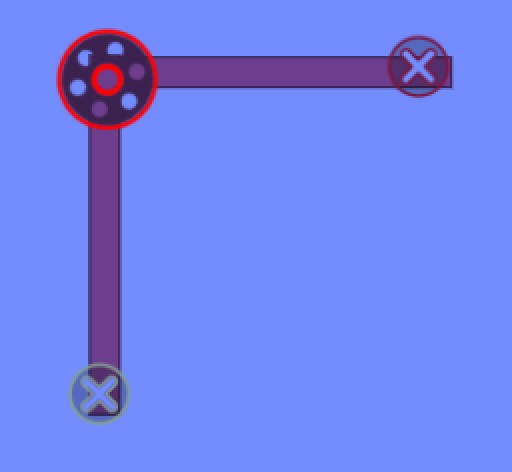
\includegraphics[width = 0.2\textwidth]{Figures/stable_2}
  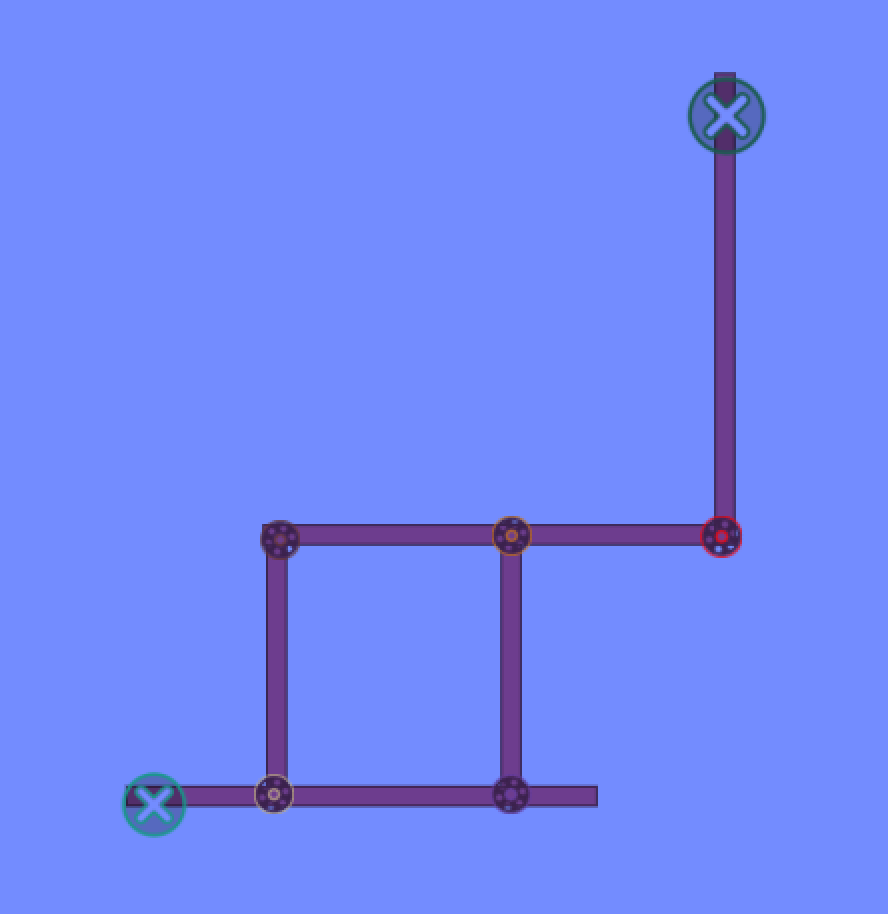
\includegraphics[width = 0.2\textwidth]{Figures/stable_3}
  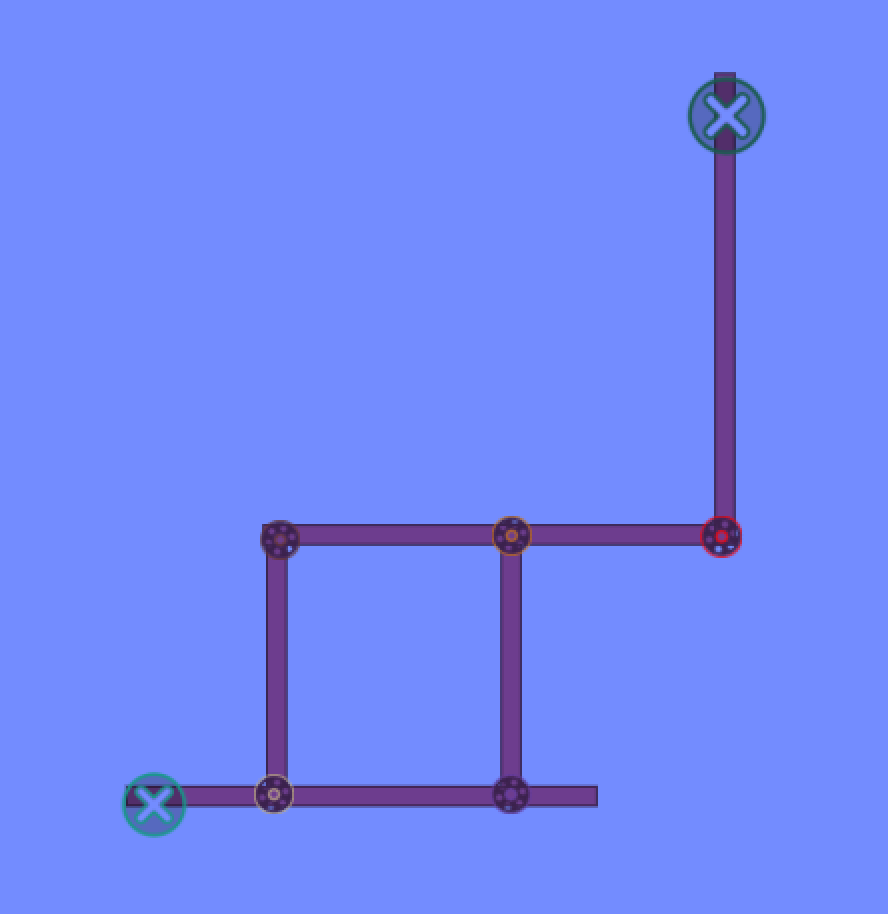
\includegraphics[width = 0.2\textwidth]{Figures/stable_4}
  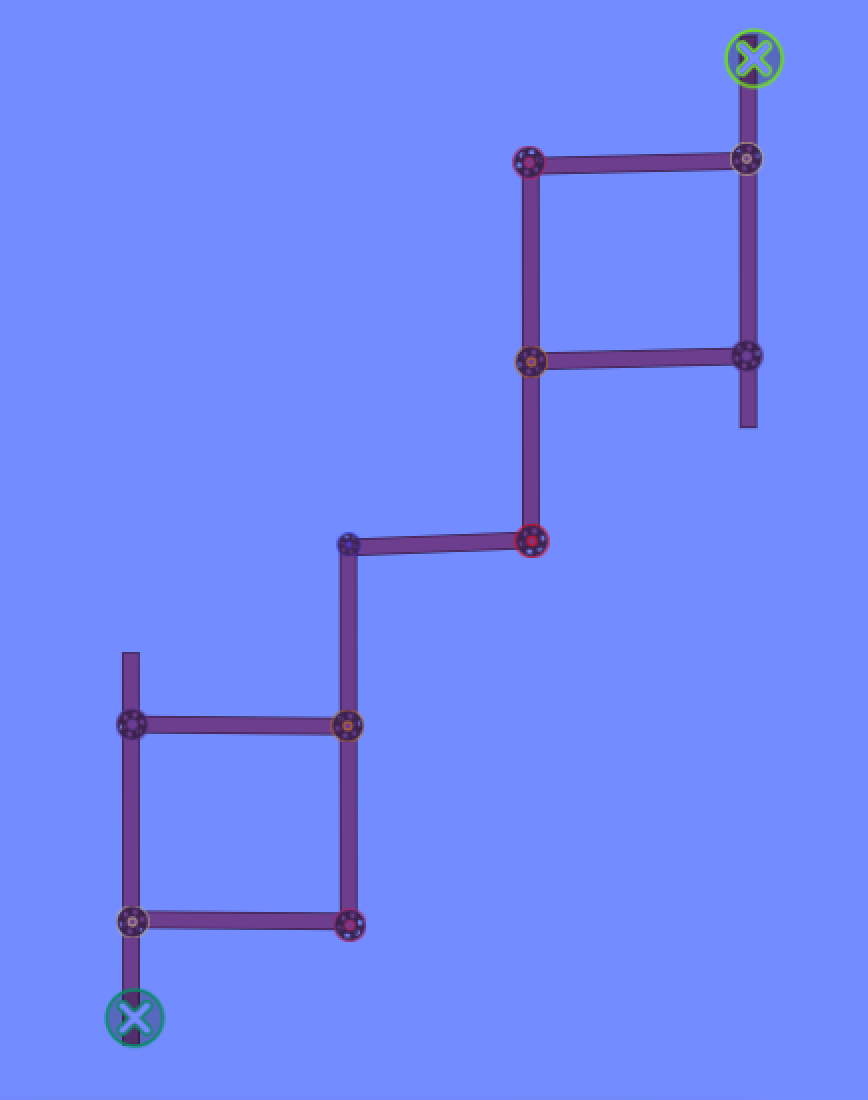
\includegraphics[width = 0.2\textwidth]{Figures/stable_5}
  \caption{The anchor with X sign represents a stable fold line and the anchor with red color is the fold line to be considered}
  \label{fig:stable}
\end{figure}

The process of determining stability is as follows:
\begin{enumerate}
\item Background fold lines are stable with stability depth 0.
\item For stability depth k, we find either the above structures based on the stable fold lines with stability depth less than k, and mark fold line in such structures as stable with stability k.
\item Repeat this process until all fold lines are marked as stable at some point. (We set a stability depth limit in practice.)
\end{enumerate}
\subsection{Consistency}
As we design the popup craft based on the input image, we want the design result to follow the input shape. Some geometry changes are avoidable since we need to add fold lines between patches, but still we want to minimize the geometry change. Although more complicated metric could be applied here, we use a simple metric to measure the geometry change. That is, the geometry change for a fold line is the amount of shift from its initial location to its final location, and the geometry change for the design result is the summation of fold line geometry changes. So the consistency is measured as: -$\lambda_{pos}\sum_f(pos(f) - pos_i(f))^2$.
\subsection{Heuristics}

Optimization \ref{equ:optimization} gives us optimized popup graph which is foldable, connected, stable and consistent with the input image. However, the optimization problem is intractable to any existing solvers in many cases due to the large number of variables and constraints (most of which are brought for the stability constraint). So instead of optimization \ref{equ:optimization} directly, we decouple the optimization process to decrease the complexity by the following two heuristics:

\textbf{Stability Constraint Decoupling: }
The stability constraint brings in $(\#f)^3$ auxilliary variables and constraints which cause the most difficulty. Our approach is to ignore stability while optimizing other terms and then check whether the returned solution satisfies the stability constraint. If the solution is not stable, we conduct the optimization again while excluding the unstable solution. We repeat the process until we find a stable solution. To find a stable solution with fewer such attempts, we guide the process by adding another objective term. Our observation is that a good popup graph design has two attributes: 1) most intersection fold lines are active as they add connections between segments which make the popup graph more intriguing and stable, and 2) a region fold line becomes active only when it is essential to make the popup graph foldable. We use $f_i$ to denote an intersection fold line and $f_r$ a region fold line, then the objective term is $max(\sum{a(f_i)} - \sum{a(f_r)})$. This term is associated with an arbitrary large weight so that it has higher priority than the consistency objective. We denote this variation of $G = optimize^t(\mathcal{G})$ as $G = optimize^t(\mathcal{G})$ indicating only topology is considered without the stability constraint.
%The stability check can also be viewed as a variation of $optimize^s(\mathcal{G})$ where only stability constraint is considered, $\mathcal{G} = {G}$ is a set contains only the popup graph we want to check, and the return value is a boolean value indicating whether the constraint holds or not.

\textbf{Child Segment: }
A child segment a segment which lies on the same plane with its parent segment and has no fold line (like the eye of the bear). Child-parent segment pair happens when two segments have different textures but are supposed to be on the same plane. A child segment has no active fold line and thus is neither connected, or stable. So we ignore child segments when optimizing the rest graph and add them back after the optimization. For this purpose, we detect segments which are enclosed by another segment. We treat them as child segments and ignore them in the optimization. Note that, such detected segments are not always real child patches (like the nose of the bear). We address this issue by simply conduct the optimization with the rest part of the graph fixed. This time, we only consider foldability constraint. We call this optimization $optimize^c(\mathcal{G})$. Users can also denote other child patches.

Putting these two heuristics together, we reach algorithm \ref{alg:optimization}.


\begin{algorithm}
  \SetAlgoLined
  \SetKwInOut{Input}{input}
  \SetKwInOut{Output}{output}
  
  \Input{A scalar image or vector image $I$}
  \Output{A foldable, connected and stable graph design which is consistent with the input image or a failure flag.}
  Initialization: $\mathcal{G} = buildPopupGraphSet(I)$

   $\mathcal{G}' = \{G | G \in \mathcal{G} \quad and \quad \text{G has no child patch\}}$;\\
   $max\_iters = 10, iter = 0$;\\
   \While{true}{
     $G^t = optimize^t(\mathcal{G}')$;\\
     \If{$stable(G^t)$}{
       break{};\\
     }
    $\mathcal{G'} = \mathcal{G'} \ G^t$;\\
    $iter = iter + 1$;\\
    \If{$iter > max\_iters$}{
      \Return{FAILURE};
    }
  }
  $\mathcal{G}^t = \{G \approx G^t | G \in \mathcal{G}\}$;\\
  $G^{OPT} = optimize^c(\mathcal{G}^t)$;\\
  \Return{$G^{OPT}$};
  \caption{Popup Graph Optimization}
\end{algorithm}

\section{Results}

Current results delete some island patches like eyes for both cases. The island patches can be added back after the rest part is optimized. We haven't done that part yet.

\begin{figure*}[h]
  
\includegraphics[width = 0.3\textwidth]{Figures/bear/bear_ill}
  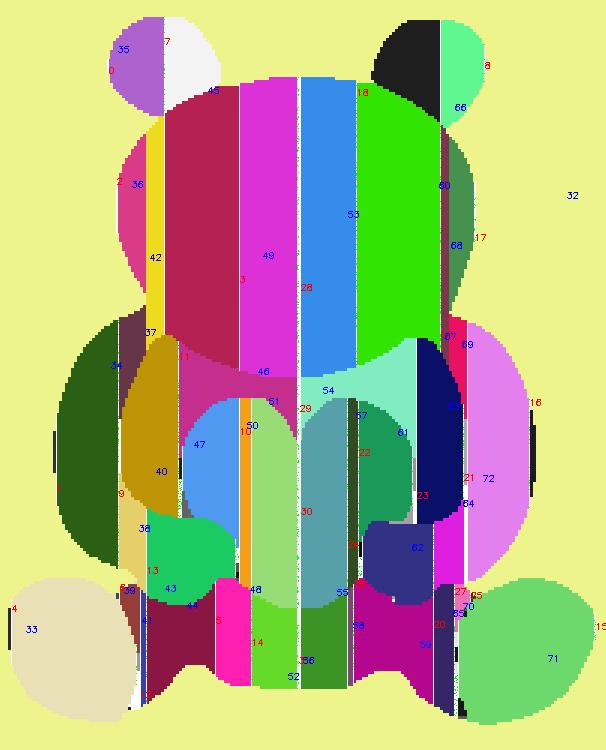
\includegraphics[width = 0.3\textwidth]{Figures/bear/popup_graph}
  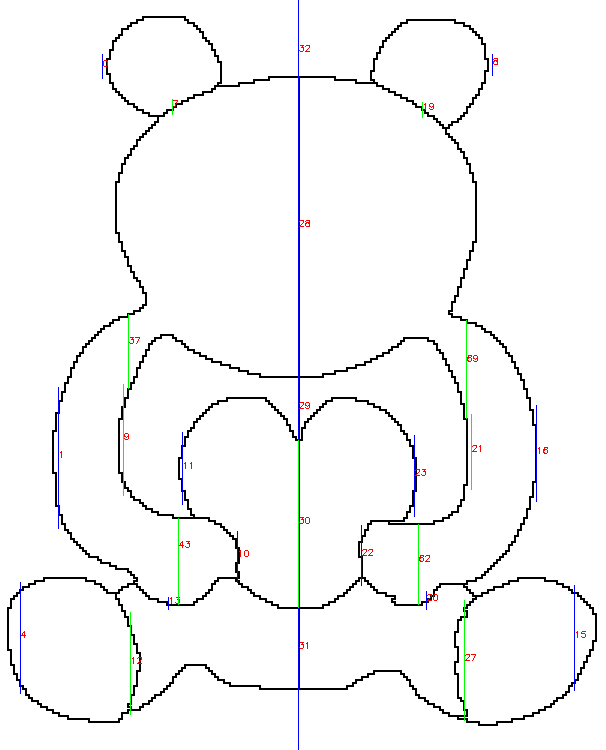
\includegraphics[width = 0.3\textwidth]{Figures/bear/optimized_popup_graph}
  \caption{Bear example: (a) input shape (b) fold line candidates (c) popup design}
  \label{fig:stable}
\end{figure*}

\begin{figure*}[h]
  
\includegraphics[width = 0.3\textwidth]{Figures/angrybird/angrybird}
  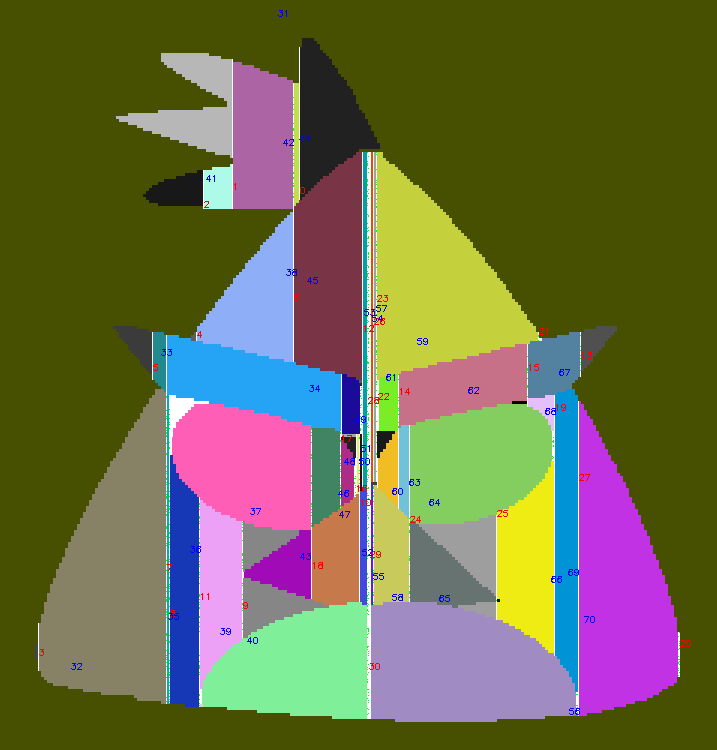
\includegraphics[width = 0.3\textwidth]{Figures/angrybird/popup_graph}
  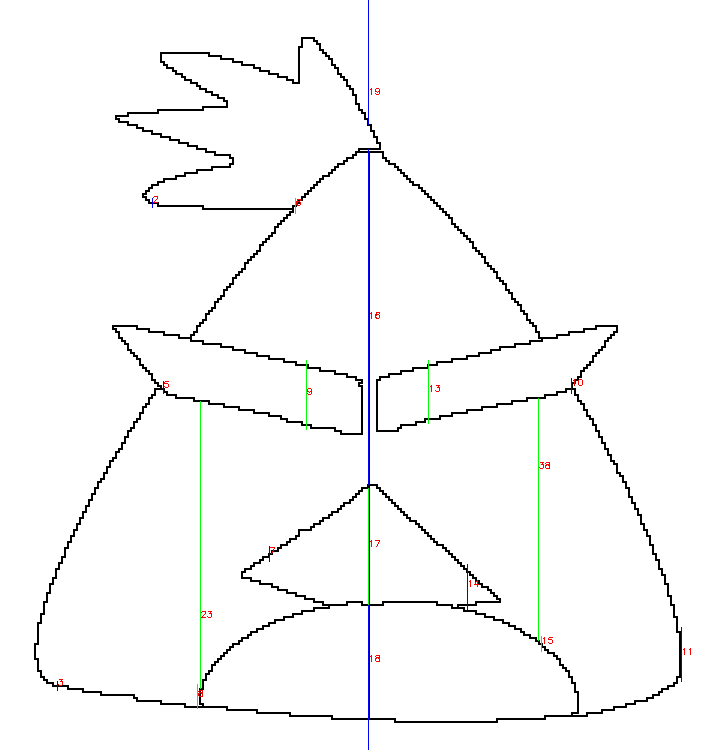
\includegraphics[width = 0.3\textwidth]{Figures/angrybird/optimized_popup_graph}
  \caption{Angrybird example: (a) input shape (b) fold line candidates (c) popup design}
  \label{fig:stable}
\end{figure*}

\section{Conclusion}
To our knowledge, this is the first work to design image-based pop-up craft via optimization.


\bibliographystyle{acmsiggraph}
\nocite{*}
\bibliography{references}
\end{document}

